\documentclass[12pt]{ctexart}
\usepackage{amsmath} % 用于数学公式
\usepackage{graphicx} % 用于插入图片
\usepackage{listings} % 用于插入代码
\usepackage{float}    % 用于控制图表浮动位置

\usepackage{booktabs} % 用于创建更美观的三线表
\usepackage{siunitx}  % 用于标准地排版物理单位和数值
\usepackage{amsmath}  % 用于数学公式环境
\sisetup{per-mode=symbol} % 设置单位格式，例如 m/s

\usepackage{fancyhdr}   % 用于自定义页眉页脚
\usepackage{caption}   % 用于自定义图表标题
\usepackage{subcaption} % 用于子图环境
\usepackage[colorlinks, linkcolor=black]{hyperref}  % 用于创建超链接
\usepackage{makecell}
\usepackage{multirow}  

% \pdfcompresslevel=9

\graphicspath{{./figures/}}

\usepackage[left=2.5cm, right=2.5cm, top=2cm, bottom=2cm]{geometry}

\setlength{\jot}{6pt} % 增加多行公式之间的行距

\linespread{1.5}

\pagestyle{fancy}

\begin{document}

% \maketitle
\thispagestyle{empty}

\begin{figure}[t]
    \centering
    
\includegraphics[width=13cm]{./figures/logo1.png}
\end{figure}

\vspace*{\fill}
    \begin{center}
        \Huge\textbf{实验6：信号的分解与合成}
    \end{center}
\vspace*{\fill}

\begin{table}[H]
    \centering
    \large
    \begin{tabular}{ll}
    \textbf{课程:} & 信号与系统实验 \\
    \textbf{姓名:} & 郭浩然 \\
    \textbf{学号:} & 2024303980 \\
    \textbf{桌号:} & 18 \\
    \textbf{班级:} & 10班 \\
    \textbf{学院:} & 民航学院 \\
    \textbf{专业:} & 飞行器控制与信息工程 \\
    \textbf{时间:} & \today \\
    \end{tabular}
\end{table}

\newpage

\tableofcontents
\newpage

% ----------------------------------------------------------------------
% 第一部分：实验目的
% ----------------------------------------------------------------------
\section{实验目的}
\begin{enumerate}
    \item 了解和熟悉波形分解与合成的原理。
    \item 了解和掌握用傅里叶级数进行谐波分析的方法。
\end{enumerate}
% ----------------------------------------------------------------------
% 第二部分：实验器材
% ----------------------------------------------------------------------
\section{实验器材}
\begin{table}[H]
    \centering
    \caption{实验器材列表}
    \begin{tabular}{clc}
        \toprule
        \textbf{序号} & \textbf{器材名称} & \textbf{数量} \\
        \midrule
        1 & 双踪示波器 & 1台 \\
        2 & 数字万用表 & 1台 \\
        3 & 信号源及频率计模块 (S2模块) & 1块 \\
        4 & 数字信号处理模块 (S4模块) & 1块 \\
        \bottomrule
    \end{tabular}
\end{table}
% ----------------------------------------------------------------------
% 第三部分：实验原理
% ----------------------------------------------------------------------
\section{实验原理}
\subsection{信号的频谱}
满足狄利克雷条件的周期信号 $f(t)$ 可展开为傅里叶级数。对于周期为 $T$ 的信号，其三角形式展开为：
\begin{equation}
    f(t) = a_0 + \sum_{n=1}^{\infty} (a_n \cos n\Omega t + b_n \sin n\Omega t)
\end{equation}
其中 $\Omega = \frac{2\pi}{T}$。通过将信号分解为直流分量及各次谐波分量，可以研究其频谱分布。
\subsection{方波信号的分解}
对于幅度为 $A$，占空比为 $50\%$ 的方波信号，其傅里叶级数展开式仅包含奇次谐波：
\begin{equation}
    f(t) = \frac{4A}{\pi} \left( \sin \omega t + \frac{1}{3} \sin 3\omega t + \frac{1}{5} \sin 5\omega t + \dots \right)
\end{equation}
各次谐波幅度理论值为 $V_n = \frac{4A}{n\pi}$ ($n=1,3,5\dots$)。
对于占空比为 $\tau/T$ 的矩形波，其各次谐波幅度由下式决定：
\begin{equation}
    |c_n| = \frac{2A}{n\pi} |\sin(n\pi \cdot \frac{\tau}{T})| \times 2 = \frac{4A}{n\pi} |\sin(n\pi \cdot \frac{\tau}{T})|
\end{equation}

\subsection{三角波信号的分解}
三角波信号的傅里叶级数展开式为：
\begin{equation}
    f(t) = \frac{8A}{\pi^2} \sum_{n=1,3,5\dots}^{\infty} \frac{1}{n^2} \cos(n\omega t)
\end{equation}
其谐波幅度随 $1/n^2$ 衰减，收敛速度快于方波。
% ----------------------------------------------------------------------
% 第四部分：实验步骤
% ----------------------------------------------------------------------
\section{实验步骤}
\subsection{任务一：方波的分解}
\begin{enumerate}
    \item 连接 S2 模块 P2 端口与 S4 模块 P9 端口。
    \item 设置 S2 输出幅度 2V，频率分别为 400Hz 和 600Hz 的方波（占空比分别调整为 50\% 和 40\%）。
    \item 将 S4 模块 SW1 拨至 ``00000101''，S3 拨至 ``00000000''。
    \item 使用示波器在 TP1 $\sim$ TP7 观测各次谐波，在 TP8 观测高次谐波。
\end{enumerate}
\subsection{任务二：方波的合成}
\begin{enumerate}
    \item 调节 S3 拨码开关，按照基波、基波+3次、基波+3+5次等组合控制谐波叠加。
    \item 在 TP8 处观察合成波形，并与原始信号对比。
\end{enumerate}
\subsection{任务三：三角波的分解与合成}
\begin{enumerate}
    \item 设置 S2 输出幅度 2V 的三角波（400Hz/600Hz）。
    \item 重复上述分解与合成步骤，记录数据并观察波形。
\end{enumerate}
% ----------------------------------------------------------------------
% 第五部分：实验数据与分析
% ----------------------------------------------------------------------
\section{实验数据与分析}
\subsection{方波信号分解数据}
% 表1：占空比 50%
\begin{table}[H]
    \centering
    \caption{占空比 50\% 方波信号频谱数据 ($A=2\text{V}$)}
    \label{tab:sq50}
    \begin{tabular}{lcccccccc}
        \toprule
        \textbf{谐波次数} & \textbf{1f} & \textbf{2f} & \textbf{3f} & \textbf{4f} & \textbf{5f} & \textbf{6f} & \textbf{7f} & \textbf{8f+} \\
        \midrule
        理论值 (V) & 2.55 & 0 & 0.85 & 0 & 0.51 & 0 & 0.36 & 0.65 \\
        400Hz 测量值 (V) & 2.60 & 0 & 1.12 & 0 & 0.76 & 0 & 0.64 & 0.32 \\
        600Hz 测量值 (V) & 2.60 & 0 & 1.08 & 0 & 0.76 & 0 & 0.64 & 0.32 \\
        \bottomrule
    \end{tabular}
\end{table}
% 表2：占空比 40%
\begin{table}[H]
    \centering
    \caption{占空比 40\% 方波信号频谱数据 ($A=2\text{V}$)}
    \label{tab:sq40}
    \begin{tabular}{lcccccccc}
        \toprule
        \textbf{谐波次数} & \textbf{1f} & \textbf{2f} & \textbf{3f} & \textbf{4f} & \textbf{5f} & \textbf{6f} & \textbf{7f} & \textbf{8f+} \\
        \midrule
        理论值 (V) & 2.42 & 0.75 & 0.50 & 0.61 & 0 & 0.40 & 0.21 & 0.63 \\
        400Hz 测量值 (V) & 2.56 & 1.04 & 0.80 & 0.88 & 0 & 0.72 & 0.52 & 0.32 \\
        600Hz 测量值 (V) & 2.56 & 1.04 & 0.76 & 0.92 & 0 & 0.72 & 0.56 & 0.36 \\
        \bottomrule
    \end{tabular}
\end{table}
\subsection{三角波信号分解数据}
% 表3：三角波
\begin{table}[H]
    \centering
    \caption{三角波信号频谱数据 ($A=2\text{V}$)}
    \label{tab:tri}
    \begin{tabular}{lcccccccc}
        \toprule
        \textbf{谐波次数} & \textbf{1f} & \textbf{2f} & \textbf{3f} & \textbf{4f} & \textbf{5f} & \textbf{6f} & \textbf{7f} & \textbf{8f+} \\
        \midrule
        理论值 (V) & 1.62 & 0 & 0.18 & 0 & 0.06 & 0 & 0.03 & 0.03 \\
        400Hz 测量值 (V) & 1.68 & 0 & 0.36 & 0 & 0.28 & 0 & 0.24 & 0 \\
        600Hz 测量值 (V) & 1.66 & 0 & 0.36 & 0 & 0.24 & 0 & 0.22 & 0 \\
        \bottomrule
    \end{tabular}
\end{table}


\subsection{信号分解频谱图}

% --- 第一组：400Hz 方波对比 (2张图) ---
\begin{figure}[H]
    \centering
    % 第一张：400Hz 40%
    \begin{subfigure}[b]{0.95\textwidth}
        \centering
        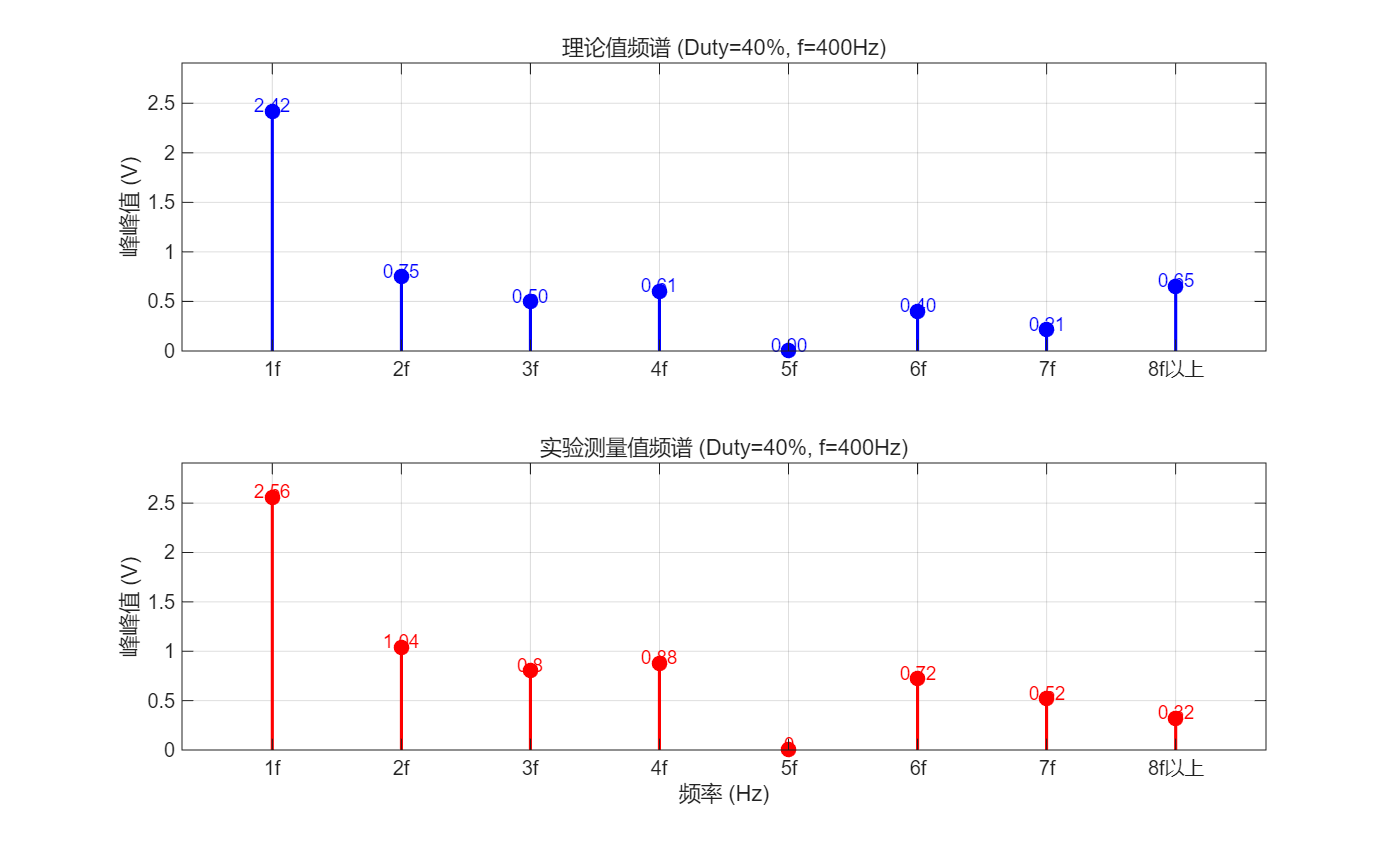
\includegraphics[width=\textwidth]{f400_40.png} 
        \caption{方波 40\% (400Hz)}
    \end{subfigure}
    
    \vspace{0.5cm} % 图片间距
    
    % 第二张：400Hz 50%
    \begin{subfigure}[b]{0.95\textwidth}
        \centering
        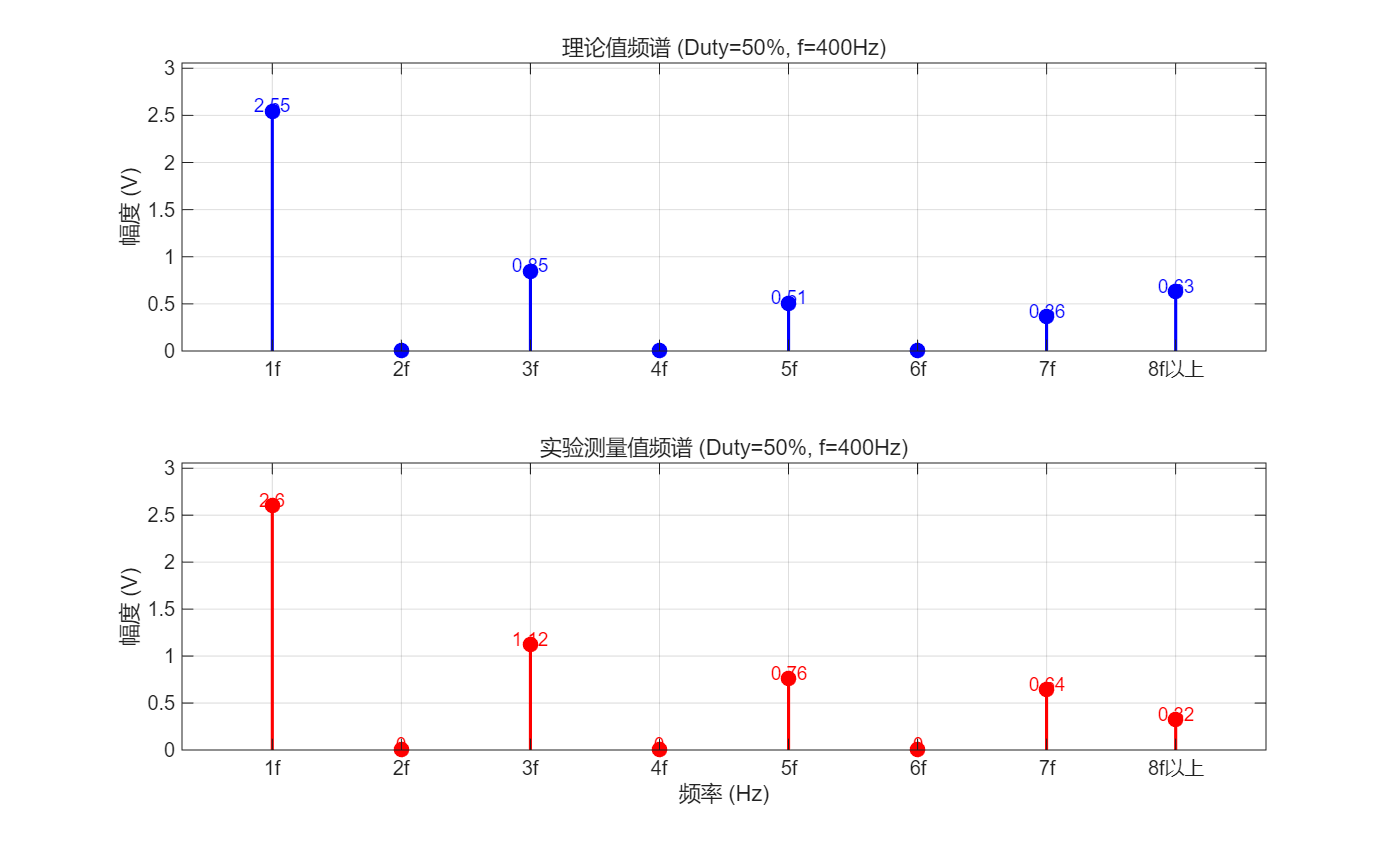
\includegraphics[width=\textwidth]{f400_50.png}
        \caption{方波 50\% (400Hz)}
    \end{subfigure}
    \caption{400Hz 方波信号频谱测量图}
\end{figure}

% --- 第二组：600Hz 方波对比 (2张图) ---
\begin{figure}[H]
    \centering
    % 第一张：600Hz 40%
    \begin{subfigure}[b]{0.95\textwidth}
        \centering
        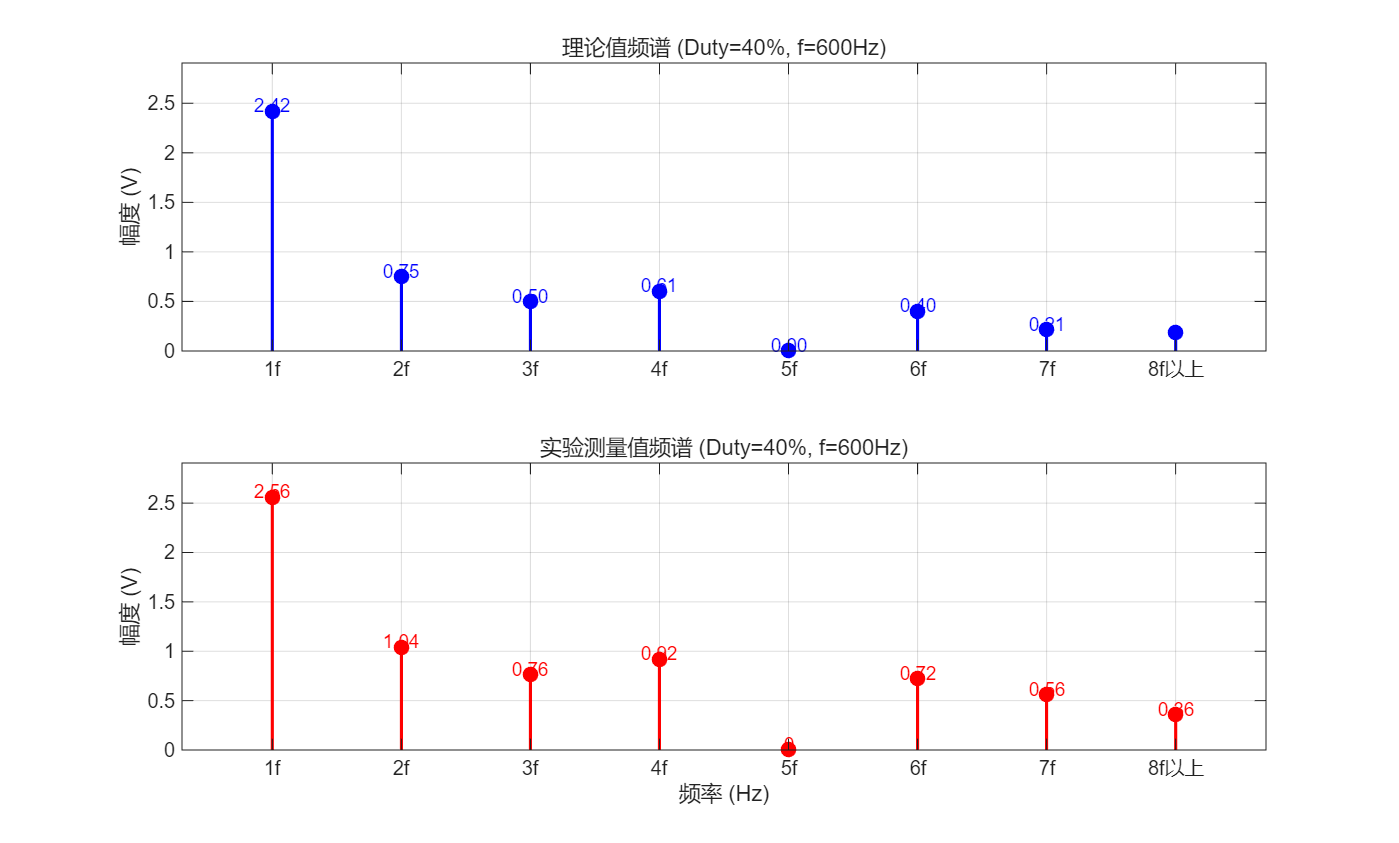
\includegraphics[width=\textwidth]{f600_40.png}
        \caption{方波 40\% (600Hz)}
    \end{subfigure}
    
    \vspace{0.5cm}
    
    % 第二张：600Hz 50%
    \begin{subfigure}[b]{0.95\textwidth}
        \centering
        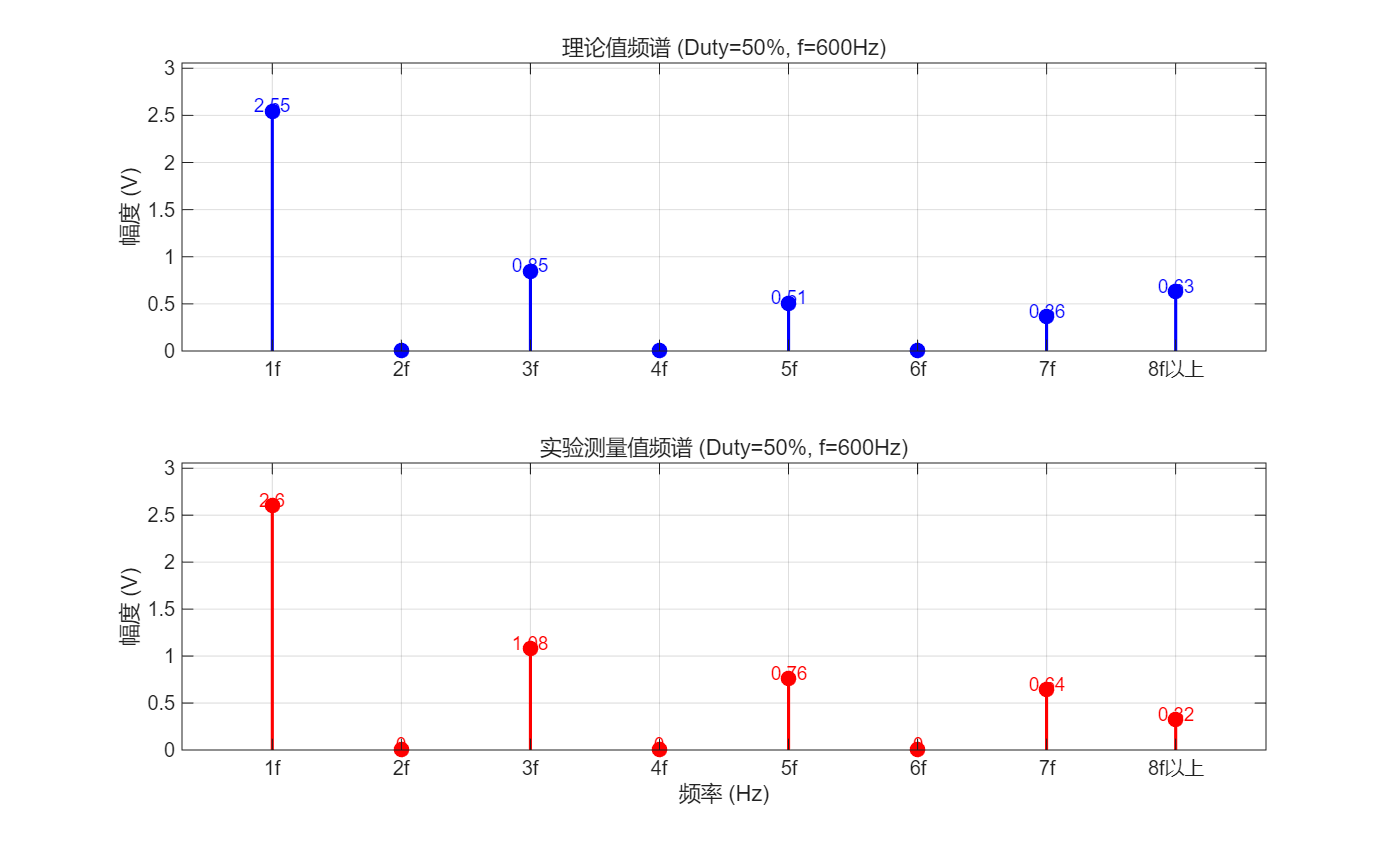
\includegraphics[width=\textwidth]{f600_50.png}
        \caption{方波 50\% (600Hz)}
    \end{subfigure}
    \caption{600Hz 方波信号频谱测量图}
\end{figure}

% --- 第三组：三角波对比 (2张图) ---
\begin{figure}[H]
    \centering
    % 第一张：400Hz 三角波
    \begin{subfigure}[b]{0.95\textwidth}
        \centering
        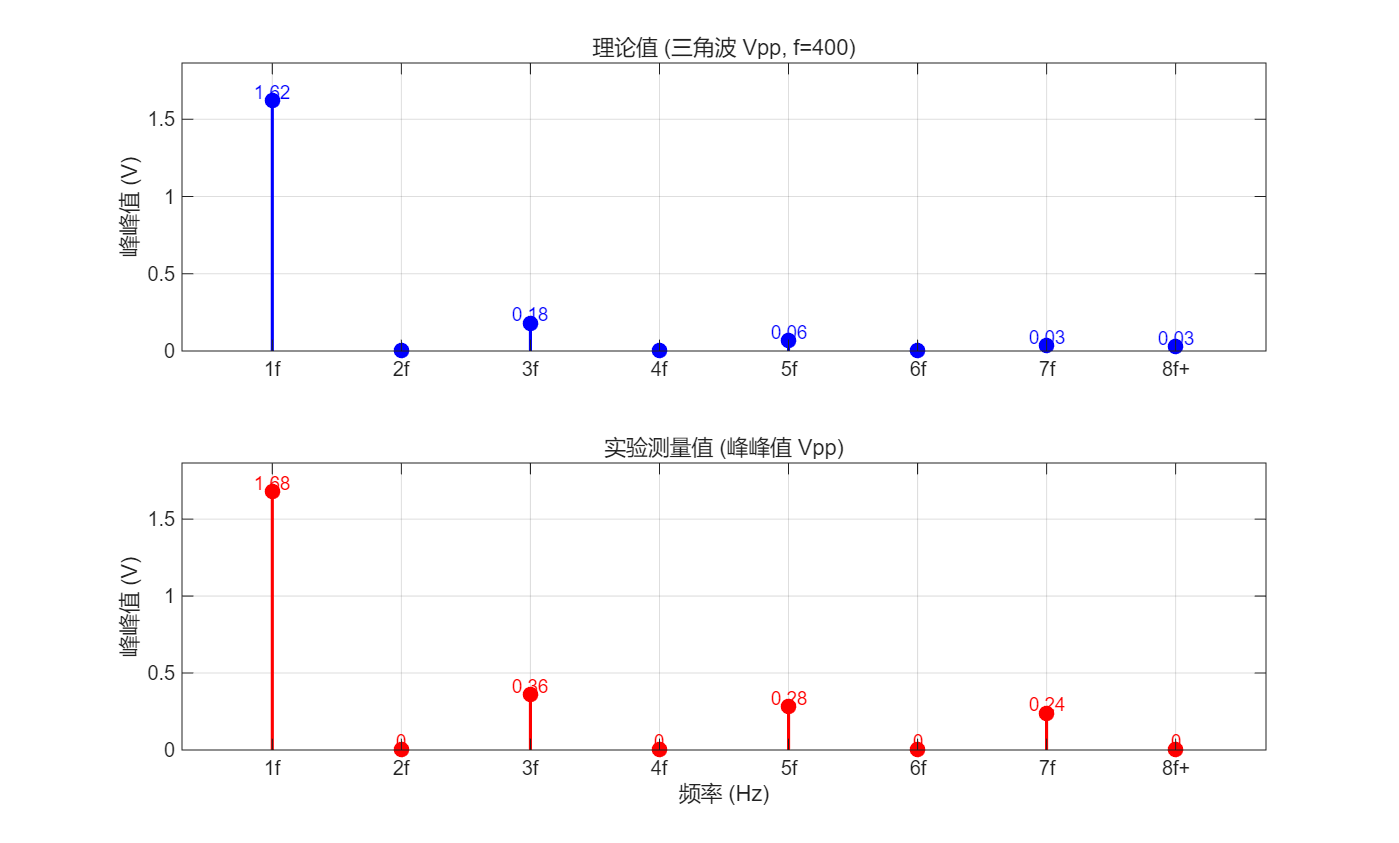
\includegraphics[width=\textwidth]{f400.png}
        \caption{三角波 (400Hz)}
    \end{subfigure}
    
    \vspace{0.5cm}
    
    % 第二张：600Hz 三角波
    \begin{subfigure}[b]{0.95\textwidth}
        \centering
        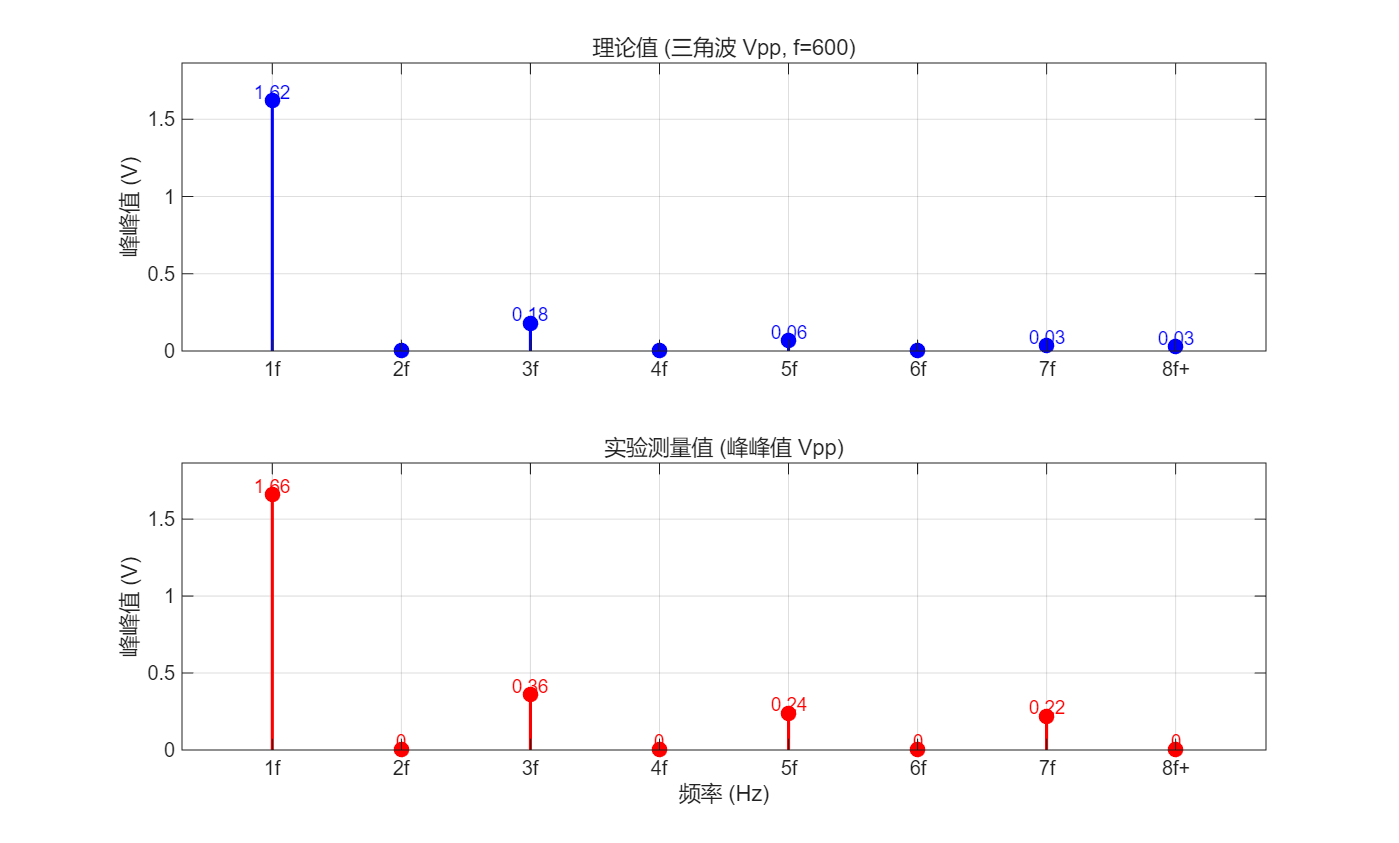
\includegraphics[width=\textwidth]{f600.png}
        \caption{三角波 (600Hz)}
    \end{subfigure}
    \caption{三角波信号频谱测量图 (400Hz 与 600Hz)}
\end{figure}


\subsubsection{方波合成 (50\% 占空比, 400Hz)}

% --- 方波合成 Part 1 (前4张) ---
\begin{figure}[H]
    \centering
    % 第一行
    \begin{subfigure}[b]{0.48\textwidth}
        \centering
        
\includegraphics[width=\textwidth]{square/1.jpg} 
        \caption{基波}
    \end{subfigure}
    \hfill
    \begin{subfigure}[b]{0.48\textwidth}
        \centering
        
\includegraphics[width=\textwidth]{square/2.jpg} 
        \caption{基波+3次谐波}
    \end{subfigure}
    
    \vspace{0.3cm}
    
    % 第二行
    \begin{subfigure}[b]{0.48\textwidth}
        \centering
        
\includegraphics[width=\textwidth]{square/3.jpg} 
        \caption{基波+5次谐波}
    \end{subfigure}
    \hfill
    \begin{subfigure}[b]{0.48\textwidth}
        \centering
        
\includegraphics[width=\textwidth]{square/4.jpg} 
        \caption{1+3+5次谐波}
    \end{subfigure}
    \caption{方波信号合成过程 (1-4步)}
\end{figure}

% --- 方波合成 Part 2 (后4张) ---
\begin{figure}[H]
    \centering
    % 第一行 (即总第3行)
    \begin{subfigure}[b]{0.48\textwidth}
        \centering
        
\includegraphics[width=\textwidth]{square/5.jpg} 
        \caption{全合成 (所有谐波)}
    \end{subfigure}
    \hfill
    \begin{subfigure}[b]{0.48\textwidth}
        \centering
        
\includegraphics[width=\textwidth]{square/6.jpg} 
        \caption{缺3次谐波}
    \end{subfigure}
    
    \vspace{0.3cm}
    
    % 第二行 (即总第4行)
    \begin{subfigure}[b]{0.48\textwidth}
        \centering
        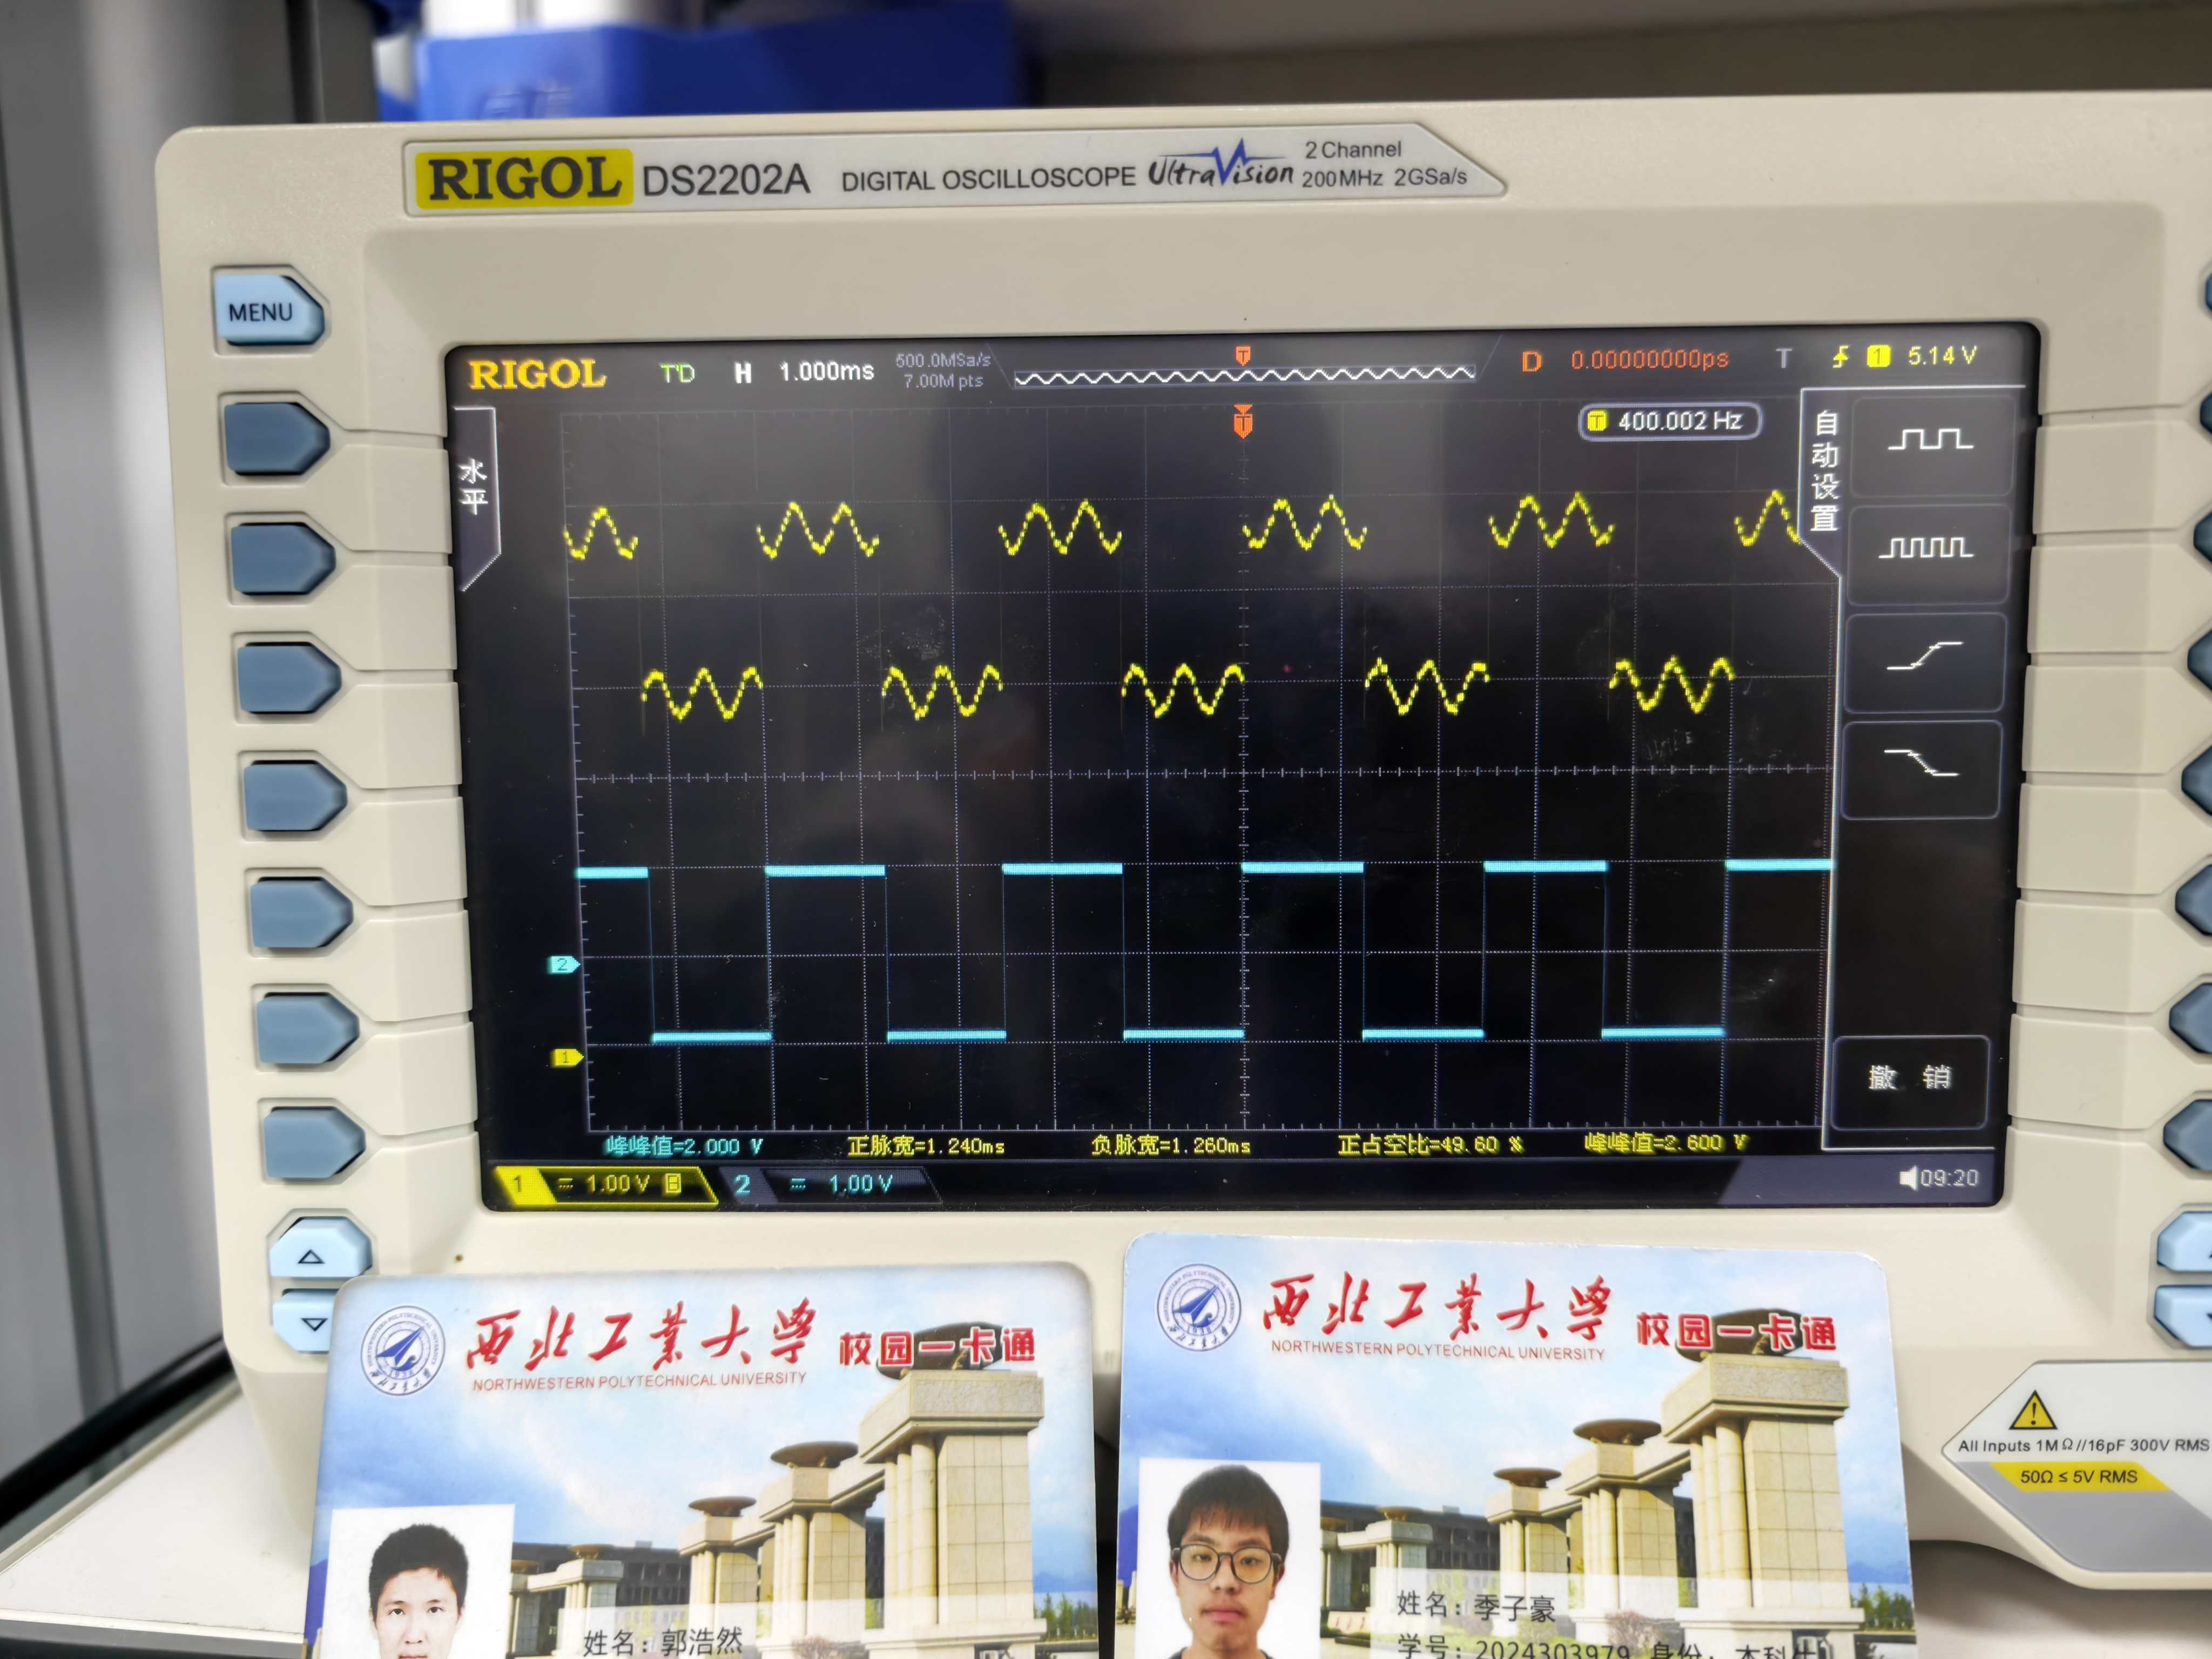
\includegraphics[width=\textwidth]{square/7.jpg} 
        \caption{缺5次谐波}
    \end{subfigure}
    \hfill
    \begin{subfigure}[b]{0.48\textwidth}
        \centering
        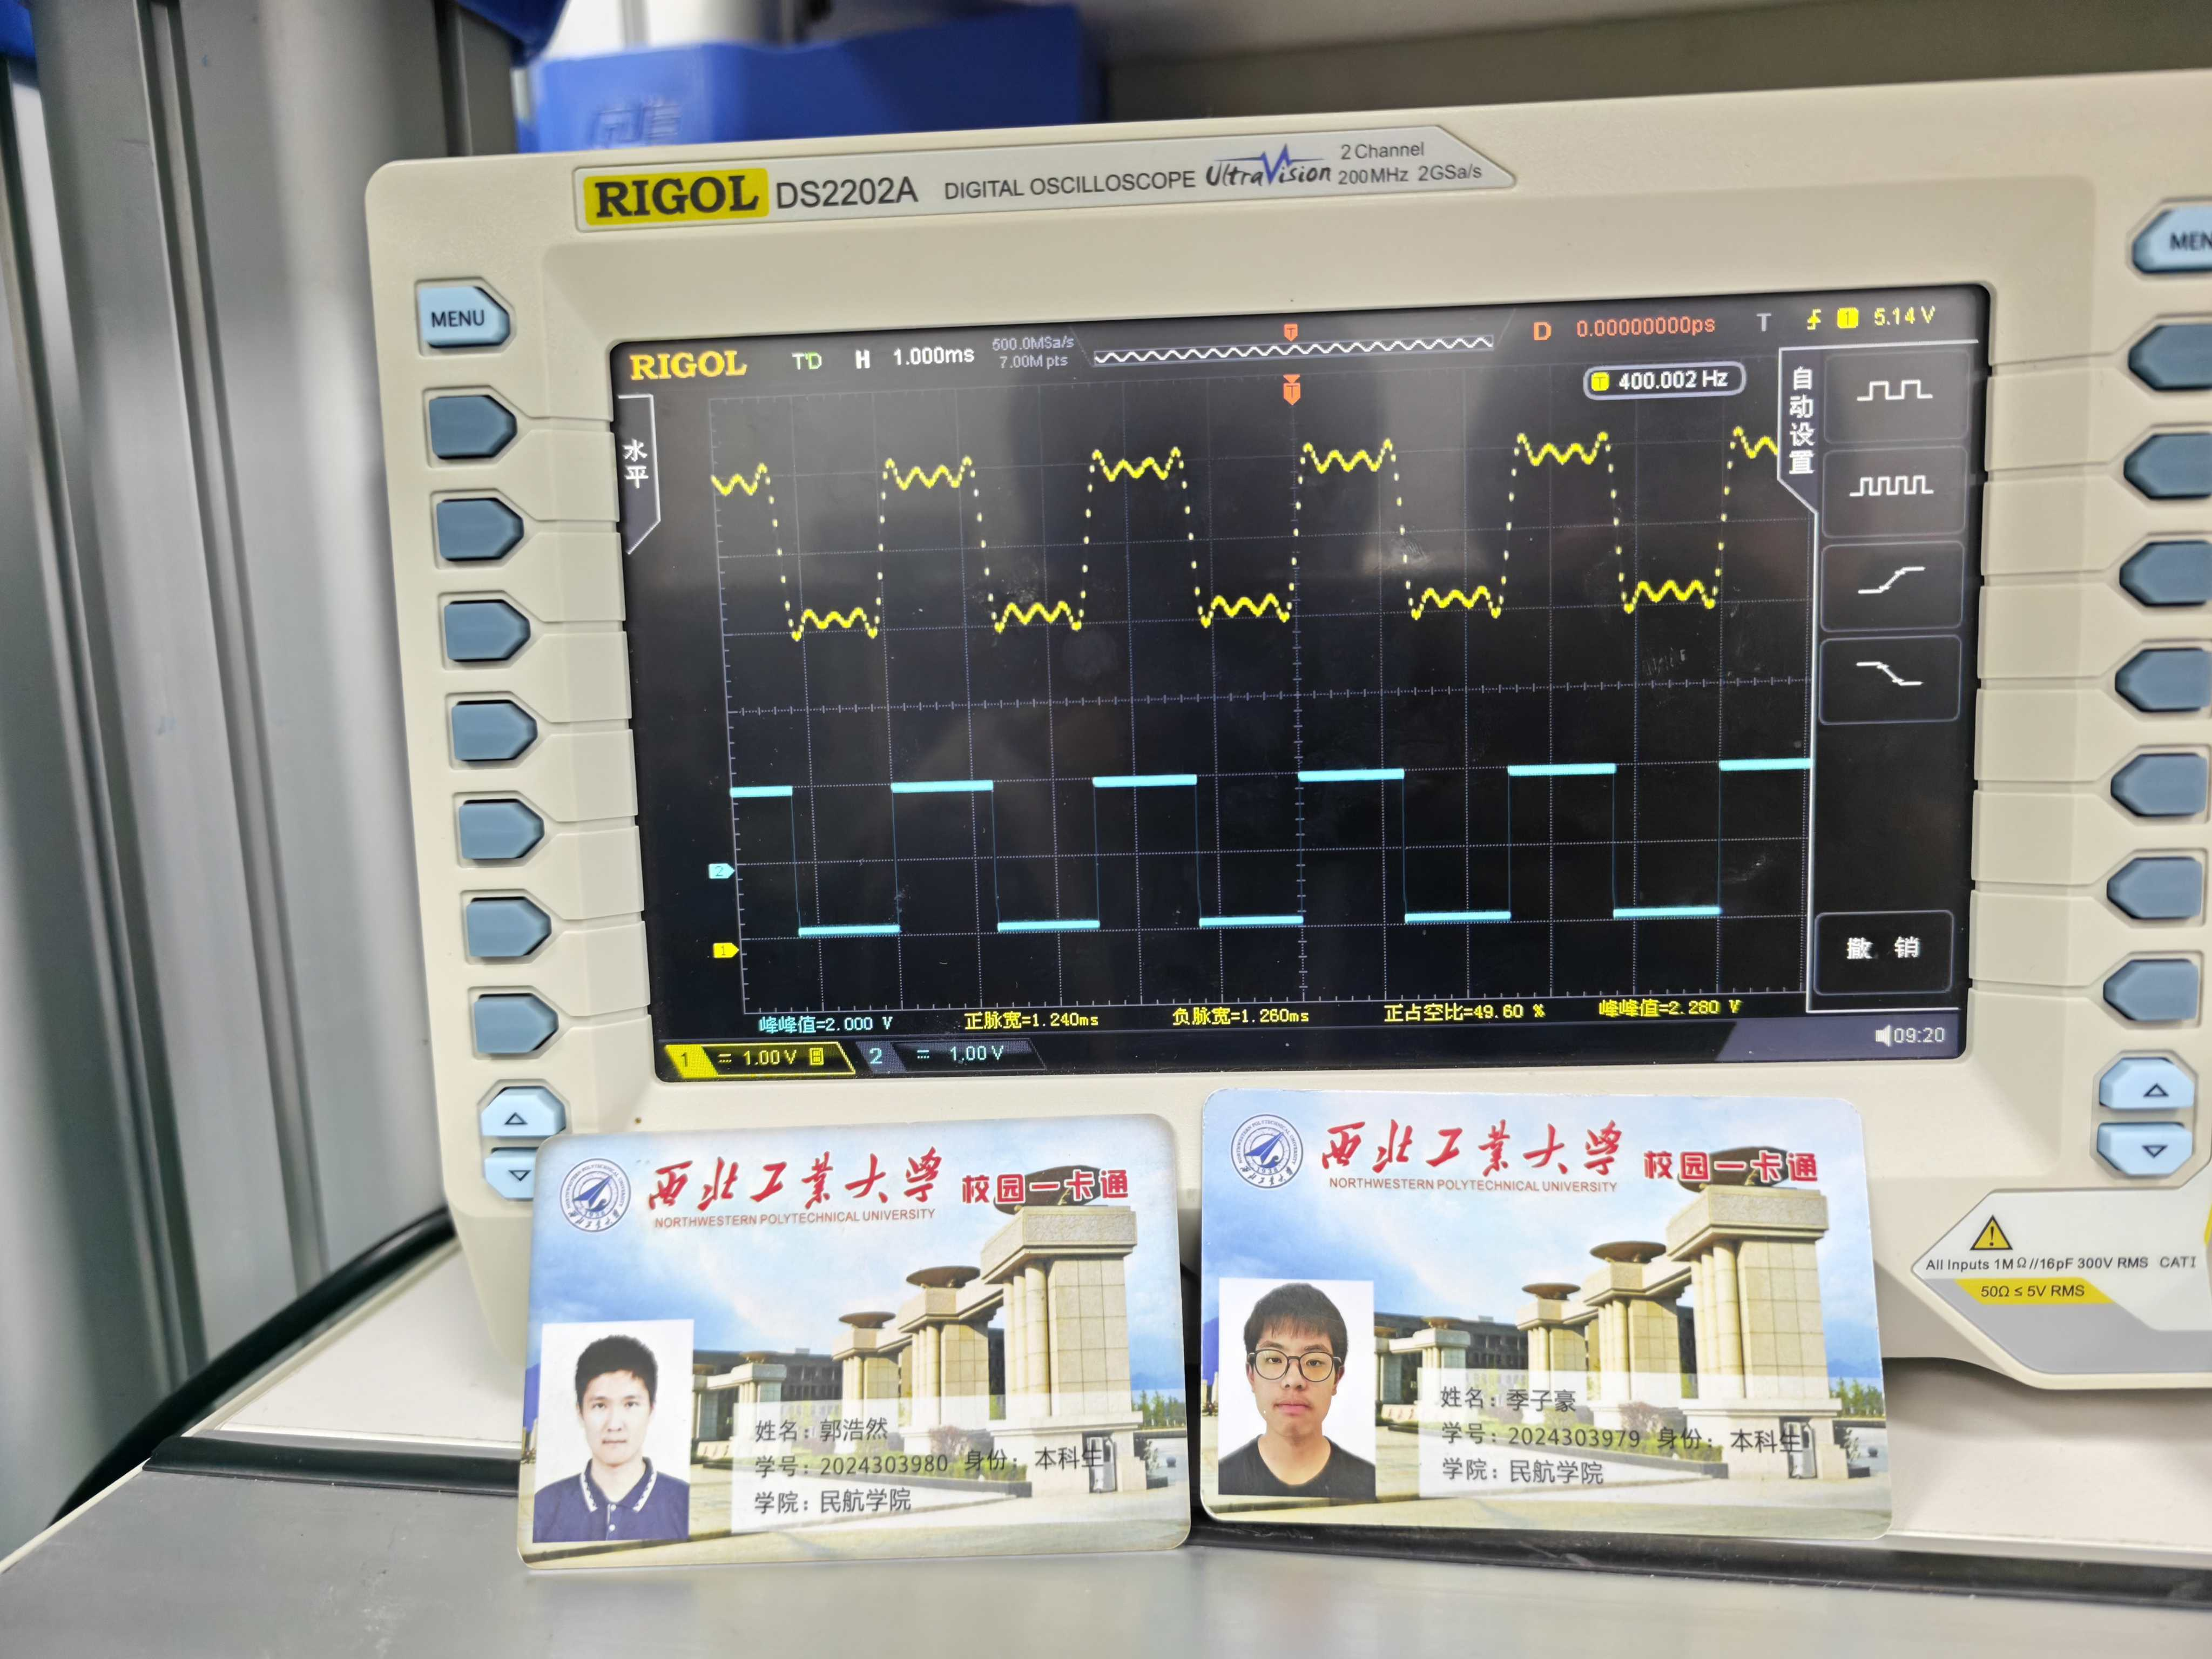
\includegraphics[width=\textwidth]{square/8.jpg} 
        \caption{缺8次以上高次谐波}
    \end{subfigure}
    \caption{方波信号合成过程 (5-8步)}
\end{figure}

\subsubsection{三角波合成 (400Hz)}

% --- 三角波合成 Part 1 (前4张) ---
\begin{figure}[H]
    \centering
    \begin{subfigure}[b]{0.48\textwidth}
        \centering
        
\includegraphics[width=\textwidth]{tri/1.jpg} 
        \caption{基波}
    \end{subfigure}
    \hfill
    \begin{subfigure}[b]{0.48\textwidth}
        \centering
        
\includegraphics[width=\textwidth]{tri/2.jpg} 
        \caption{基波+3次谐波}
    \end{subfigure}
    
    \vspace{0.3cm}
    
    \begin{subfigure}[b]{0.48\textwidth}
        \centering
        
\includegraphics[width=\textwidth]{tri/3.jpg} 
        \caption{基波+5次谐波}
    \end{subfigure}
    \hfill
    \begin{subfigure}[b]{0.48\textwidth}
        \centering
        
\includegraphics[width=\textwidth]{tri/4.jpg} 
        \caption{1+3+5次谐波}
    \end{subfigure}
    \caption{三角波信号合成过程 (1-4步)}
\end{figure}

% --- 三角波合成 Part 2 (后4张) ---
\begin{figure}[H]
    \centering
    \begin{subfigure}[b]{0.48\textwidth}
        \centering
        
\includegraphics[width=\textwidth]{tri/5.jpg} 
        \caption{全合成 (所有谐波)}
    \end{subfigure}
    \hfill
    \begin{subfigure}[b]{0.48\textwidth}
        \centering
        
\includegraphics[width=\textwidth]{tri/6.jpg} 
        \caption{缺3次谐波}
    \end{subfigure}
    
    \vspace{0.3cm}
    
    \begin{subfigure}[b]{0.48\textwidth}
        \centering
        
\includegraphics[width=\textwidth]{tri/7.jpg} 
        \caption{缺5次谐波}
    \end{subfigure}
    \hfill
    \begin{subfigure}[b]{0.48\textwidth}
        \centering
        
\includegraphics[width=\textwidth]{tri/8.jpg} 
        \caption{缺8次以上高次谐波}
    \end{subfigure}
    \caption{三角波信号合成过程 (5-8步)}
\end{figure}

\newpage

% ----------------------------------------------------------------------
% 第六部分：实验结论
% ----------------------------------------------------------------------
\section{实验结论}
通过本次实验，得出以下结论：
\begin{enumerate}
    \item \textbf{频谱特性验证}：实验数据表明，方波（50\%占空比）和三角波主要由奇次谐波组成，偶次谐波分量接近于零，这与傅里叶级数理论分析一致。40\%占空比的方波则出现了明显的偶次谐波分量，验证了波形对称性对频谱的影响。
    \item \textbf{谐波衰减规律}：对比方波和三角波的测量数据，三角波的高次谐波幅度衰减速度明显快于方波（如3次谐波处，方波约为基波的1/3，而三角波约为基波的1/9），验证了不同波形谐波收敛速度的理论差异。
    \item \textbf{波形合成}：通过叠加不同次数的谐波，示波器观测到的合成波形逐渐逼近原始信号。随着参与合成的谐波次数增加，波形的吉布斯现象（Gibbs Phenomenon）细节和边缘陡峭度得到改善，证明了周期信号可由一系列正弦波叠加而成的原理。
    \item \textbf{误差分析}：测量值与理论值存在一定偏差（特别是高次谐波偏大），这可能源于数字滤波器模块的增益误差、信号源输出幅度的非理想性以及示波器读数误差。
\end{enumerate}

\end{document}